\chapter{Mekanika Benda Tegar}\label{ch:b2:rigid-body-mechanics}

Amatilah sebuah roda sepeda dari tepi jalan: jeruji yang dekat aspal
hampir diam dan tampak tajam, jeruji di puncaknya kabur dan melaju dua
kali lebih cepat daripada pengendaranya. Setiap titik roda mempunyai
kecepatan yang berbeda, namun rodanya satu benda --- titik-titiknya
menjaga jaraknya, dan kendala tunggal itu menata seluruh geraknya
menjadi dua vektor saja, sebuah translasi dan sebuah rotasi. Jilid Tahun
ke-1 menggarap kasus khusus \omterm{def:b2:rigid-body-mechanics:solid}{benda tegar} yang berputar terhadap sumbu
tetap; bab ini menyajikan kinematika umum sebuah \omterm{def:b2:rigid-body-mechanics:solid}{benda tegar}, energi
kinetik dan momentum sudutnya, hukum-hukum geraknya, dan hukum yang
mengatur setiap roda, ban, rem dan tangga: hukum gesekan kering Coulomb.

\section{Kinematika benda tegar}

\begin{definition}[Benda tegar]\label{def:b2:rigid-body-mechanics:solid}
\index{benda tegar}
Yang disebut \emph{benda tegar} adalah sistem titik yang jarak
antar-titiknya tetap: $\|\vect{AB}\|$ tidak bergantung pada waktu untuk
setiap pasangan titik $A$, $B$ miliknya. Kerangka yang di dalamnya setiap
titik benda tegar itu diam disebut \emph{kerangka terpaut benda}.
\end{definition}

\begin{theorem}[Medan kecepatan benda tegar]\label{thm:b2:rigid-body-mechanics:field}
\index{vektor rotasi}\index{medan kecepatan (benda tegar)}
Pada setiap saat terdapat sebuah vektor $\vect\Omega$, yang disebut
\emph{\omterm{thm:b2:rigid-body-mechanics:field}{vektor rotasi}} \omterm{def:b2:rigid-body-mechanics:solid}{benda tegar} itu (satuan \unit{rad/s}), sedemikian
sehingga kecepatan sepasang titiknya $A$ dan $M$ dalam kerangka $\mathcal R$ memenuhi
\[
\vect v_M = \vect v_A + \vect\Omega\wedge\vect{AM} .
\]
$\vect\Omega$ tidak bergantung pada pilihan $A$; sebuah vektor $\vect u$
yang terpaut pada \omterm{def:b2:rigid-body-mechanics:solid}{benda tegar} berubah menurut $\dd\vect u/\dd t = \vect\Omega\wedge\vect u$.
\end{theorem}

\begin{proof}
Misalkan $(\vect e_1, \vect e_2, \vect e_3)$ basis ortonormal yang terpaut
pada \omterm{def:b2:rigid-body-mechanics:solid}{benda tegar}. Dari $\vect e_i\cdot\vect e_j = \delta_{ij}$, koefisien
$a_{ij} = \dot{\vect e}_i\cdot\vect e_j$ memenuhi $a_{ij} + a_{ji} = 0$:
matriks pemetaan $\vect u \mapsto \dot{\vect u}$ (untuk $\vect u$ yang
terpaut pada bendanya, $\vect u = \sum u_i\vect e_i$ dengan $u_i$ tetap)
bersifat antisimetrik, dan matriks antisimetrik $3\times3$ adalah matriks
$\vect u \mapsto \vect\Omega\wedge\vect u$ dengan $\Omega_1 = a_{23}$,
$\Omega_2 = a_{31}$, $\Omega_3 = a_{12}$. Terapkanlah pada $\vect u =
\vect{AM}$: $\vect v_M - \vect v_A = \vect\Omega\wedge\vect{AM}$. Jika
$\vect\Omega'$ melakukan hal yang sama, maka $(\vect\Omega - \vect\Omega')\wedge
\vect{AM} = \vect 0$ untuk setiap $M$, sehingga $\vect\Omega' = \vect\Omega$.
\end{proof}

\begin{remark}[Tiga macam gerak]\label{rem:b2:rigid-body-mechanics:motions}
\index{translasi}\index{rotasi terhadap sumbu tetap}
\emph{Translasi}: $\vect\Omega = \vect 0$, semua titik berbagi satu
kecepatan (tidak harus gerak lurus: kabin bianglala bertranslasi pada
sebuah lingkaran). \emph{\omterm{rem:b2:rigid-body-mechanics:motions}{Rotasi terhadap sumbu tetap}} $\Delta$:
titik-titik $\Delta$ diam, $\vect\Omega = \omega\,\vect e_\Delta$, dan
sebuah titik yang berjarak $r$ dari sumbunya bergerak pada lingkaran
dengan kelajuan $r|\omega|$ --- kasus jilid Tahun ke-1. Gerak umumnya
memadukan keduanya: $\vect v_M = \vect v_G + \vect\Omega\wedge\vect{GM}$,
sebuah translasi dengan kecepatan pusat massa ditambah sebuah rotasi
terhadap $G$.
\end{remark}

\begin{definition}[Menggelinding tanpa selip]\label{def:b2:rigid-body-mechanics:rolling}
\index{menggelinding tanpa selip}\index{kecepatan selip}
Dua \omterm{def:b2:rigid-body-mechanics:solid}{benda tegar} $S_1$ dan $S_2$ bersentuhan di sebuah titik $I$. Yang
disebut \emph{kecepatan selip} $S_1$ terhadap $S_2$ adalah $\vect v_{\text{selip}} = \vect v_{I \in S_1}
- \vect v_{I \in S_2}$, selisih kecepatan dua titik materi yang berimpit
di $I$ pada saat itu. $S_1$ \emph{menggelinding tanpa selip} pada $S_2$
apabila $\vect v_{\text{selip}} = \vect 0$. Untuk sebuah roda berjari-jari
$R$ yang menggelinding tanpa selip di atas lantai tetap, dengan kecepatan
pusat $v_G$ dan kecepatan sudut $\omega$, syaratnya berbunyi
$v_G = R\omega$ (tandanya dipilih sehingga roda yang menggelinding ke
kanan berputar searah jarum jam).
\end{definition}

\begin{proof}
Terapkanlah \cref{thm:b2:rigid-body-mechanics:field} pada rodanya antara
$G$ dan titik sentuh $I$: $\vect v_{I\in S_1} = \vect v_G + \vect\Omega
\wedge\vect{GI}$; dengan $\vect v_G = v_G\vect e_x$, $\vect\Omega = -\omega
\vect e_z$ dan $\vect{GI} = -R\vect e_y$, ini sama dengan $(v_G - R\omega)\vect e_x$,
yang harus lenyap.
\end{proof}

\begin{example}[Medan kecepatan roda yang menggelinding]\label{ex:b2:rigid-body-mechanics:wheel}
Untuk roda yang menggelinding, $\vect v_M = \vect\Omega\wedge\vect{IM}$:
pada setiap saat rodanya \emph{berputar terhadap titik sentuhnya}. Titik
sentuhnya diam, pusatnya bergerak dengan $v = R\omega$, puncaknya dengan
$2v$, dan sebuah titik pelek pada ketinggian $h$ bergerak dengan
$\omega\sqrt{2Rh}$, tegak lurus $\vect{IM}$. Pentil roda melukiskan
sebuah sikloida; batu yang terlempar dari tapak ban meninggalkannya
dengan kelajuan titik pelek, sampai $2v$ --- itulah sebabnya penahan
lumpur sebuah truk penting.
\end{example}

\begin{omfigure}
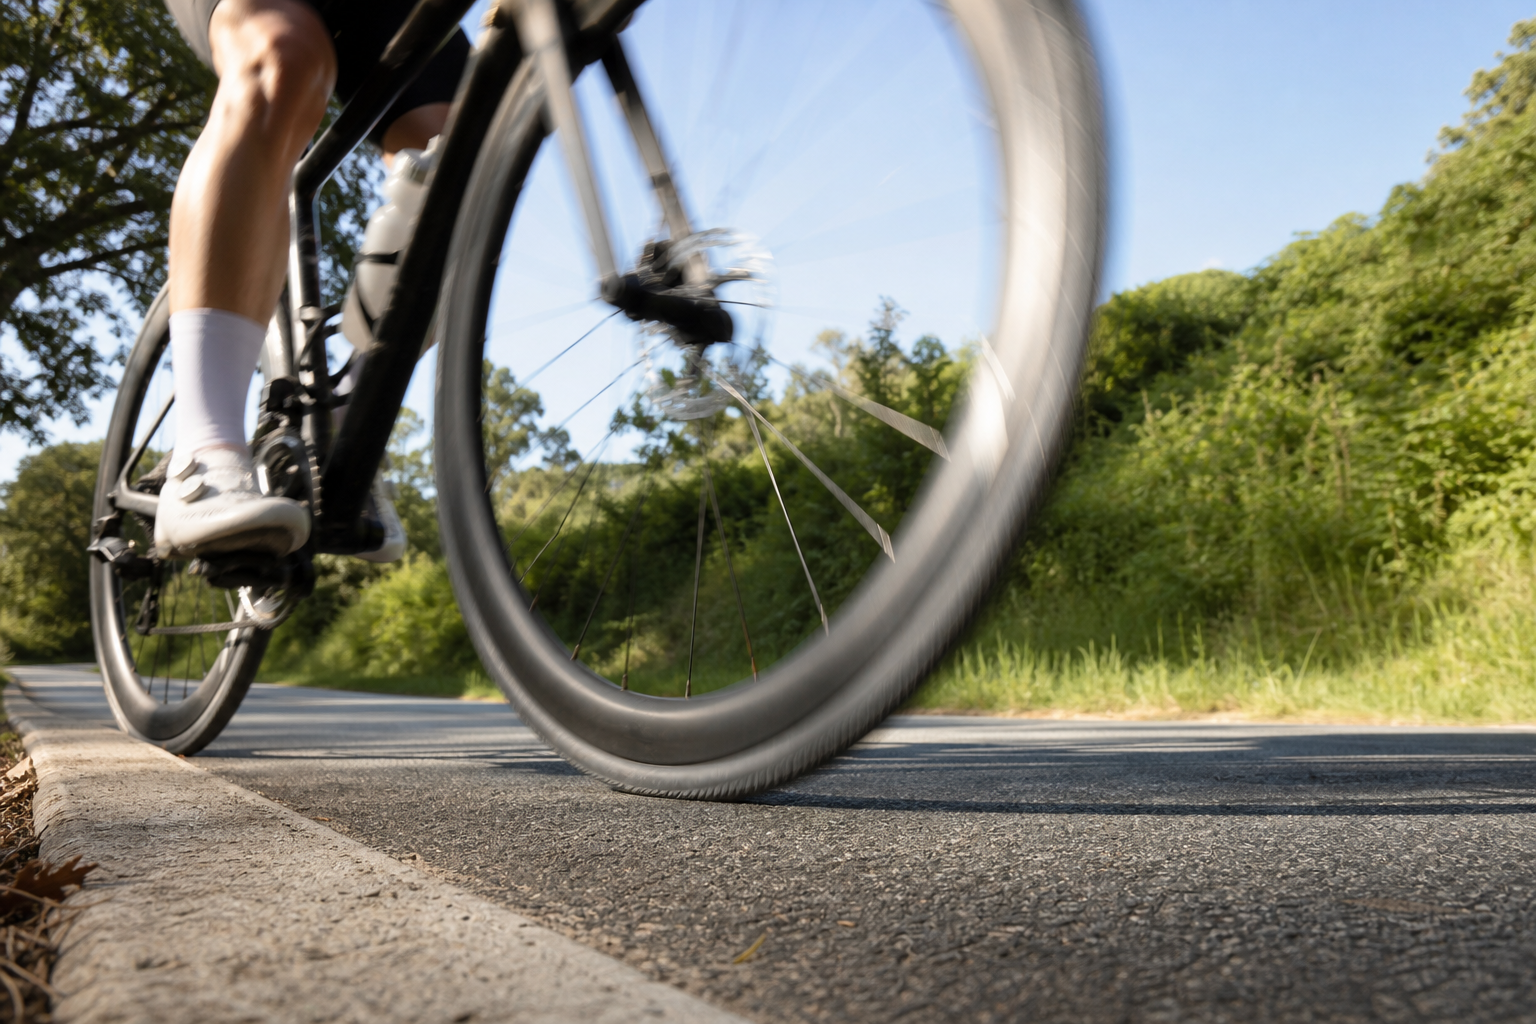
\includegraphics[width=0.58\linewidth]{images/book4/ai/b4-01-bicycle-wheel-blur.png}

{\small Sebuah roda yang tertangkap rana lambat: jeruji dekat jalan, yang hampir diam, tetap tajam; jeruji di puncaknya, yang melaju dua kali kelajuan sepedanya, menjadi kabur.}
\end{omfigure}


\begin{omfigure}
\begin{tikzpicture}[font=\small, x=1cm, y=1cm, >=Stealth]
  \begin{scope}
    \draw[thick] (-2.6,0) -- (2.6,0);
    \draw[omDef, thick] (0,1.5) circle (1.5);
    \fill (0,1.5) circle (1.5pt) node[below left, font=\footnotesize] {$G$};
    \fill (0,0) circle (1.5pt) node[below, font=\footnotesize] {$I$};
    \draw[omThm, very thick, ->] (0,1.5) -- (1.2,1.5) node[above, font=\footnotesize] {$\vect v_G$};
    \draw[omThm, very thick, ->] (0,3.0) -- (2.4,3.0) node[pos=0.35, above, font=\footnotesize] {$2\vect v_G$};
    \draw[omThm, very thick, ->] (1.5,1.5) -- (2.7,0.3) node[right, font=\footnotesize] {$\sqrt2\,v_G$};
    \draw[omThm, very thick, ->] (-1.5,1.5) -- (-0.3,2.7) node[above left, font=\footnotesize] {$\sqrt2\,v_G$};
    \draw[omThm, thick, ->] (1.06,0.44) -- (1.41,-0.41);
    \draw[omThm, thick, ->] (-1.06,0.44) -- (-0.71,1.29);
    \node[omThm, font=\footnotesize] at (0.3,0.35) {$\vect v_I = \vect 0$};
    \draw[omProp, ->] (-0.5,2.1) arc[start angle=130, end angle=50, radius=0.75] node[midway, above, font=\footnotesize] {$\omega$};
  \end{scope}
  \begin{scope}[xshift=7.6cm]
    \draw[thick] (-2.6,0) -- (2.6,0);
    \draw[omDef, thick] (0,1.5) circle (1.5);
    \fill (0,0) circle (1.5pt) node[below, font=\footnotesize] {$I$};
    \fill (0,1.5) circle (1.5pt);
    \draw[omThm, ->] (0,1.5) -- ($(0,1.5)!0.45!90:(0,0)$);
    \foreach \a in {30,60,...,330} {
      \coordinate (M) at ({1.5*cos(\a)},{1.5+1.5*sin(\a)});
      \draw[omThm, ->] (M) -- ($(M)!0.45!90:(0,0)$);
    }
    \draw[dashed, omExo] (0,0) -- (1.3,2.25);
    \fill (1.3,2.25) circle (1.2pt) node[right, font=\footnotesize] {$M$};
    \node[font=\footnotesize] at (0,-0.8) {$\vect v_M = \vect\Omega\wedge\vect{IM}$};
    \node[font=\footnotesize, align=center] at (0,3.6) {rotasi seketika\\terhadap titik sentuh};
  \end{scope}
\end{tikzpicture}

{\small Sebuah roda yang \omterm{def:b2:rigid-body-mechanics:rolling}{menggelinding tanpa selip}. Kiri: kecepatan
beberapa titik --- nol di titik sentuh $I$, $v_G = R\omega$ di pusatnya,
$2v_G$ di puncaknya. Kanan: setiap kecepatan tegak lurus ruas garis yang
menghubungkan titiknya ke $I$ dan sebanding dengan panjangnya: pada
setiap saat rodanya berputar terhadap titik sentuhnya.}
\end{omfigure}

\section{Besaran kinetik sebuah benda tegar}

\begin{proposition}[Momentum, momentum sudut, energi kinetik]\label{prop:b2:rigid-body-mechanics:kinetic}
\index{momen inersia}\index{momentum sudut (benda tegar)}\index{energi kinetik (benda tegar)}
Untuk \omterm{def:b2:rigid-body-mechanics:solid}{benda tegar} bermassa $M$ dengan pusat massa $G$, dalam kerangka
$\mathcal R$:
\begin{itemize}
  \item momentumnya adalah $\vect p = M\vect v_G$;
  \item jika ia berputar terhadap sebuah sumbu $\Delta$ (tetap dalam
        $\mathcal R$, atau melalui $G$ dan tetap arahnya) dengan
        kecepatan sudut $\omega$, momentum sudutnya \emph{sepanjang}
        sumbu itu adalah $L_\Delta = J_\Delta\,\omega$, dengan
        \[
        J_\Delta = \sum_i m_i r_i^2 = \int r^2\,\dd m
        \]
        yang disebut \emph{\omterm{prop:b2:rigid-body-mechanics:kinetic}{momen inersia}} terhadap $\Delta$ ($r$ jarak
        ke sumbunya; satuan \unit{kg.m^2});
  \item energi kinetiknya adalah (Koenig) $E_k = \tfrac12Mv_G^2 +
        E_k^*$, dengan energi kinetik dalam kerangka barisentrik
        $E_k^* = \tfrac12J_{G}\omega^2$ untuk rotasi berkecepatan
        $\omega$ terhadap sumbu yang melalui $G$ --- dan
        $E_k = \tfrac12J_\Delta\omega^2$ untuk \omterm{rem:b2:rigid-body-mechanics:motions}{rotasi terhadap sumbu
        tetap} $\Delta$.
\end{itemize}
\end{proposition}

\begin{proof}
Teorema momentum dan teorema Koenig telah dibuktikan dalam jilid Tahun
ke-1 untuk sembarang sistem. Untuk rotasi terhadap $\Delta$ yang melalui
$O$, sebuah titik berjarak $r_i$ dari sumbunya berkelajuan $r_i\omega$
pada lingkaran mengelilingi sumbu itu; momentum sudutnya terhadap $O$
yang diproyeksikan pada $\vect e_\Delta$ adalah $m_ir_i^2\omega$
(komponen lainnya, yang saling meniadakan pada benda simetrik, tidak
diperlukan di sini); jumlahkan. Energi kinetik: $\sum\tfrac12m_ir_i^2
\omega^2$.
\end{proof}

\begin{remark}[Yang diterima tanpa bukti]\label{rem:b2:rigid-body-mechanics:tensor}
Untuk rotasi $\vect\Omega$ sembarang, vektor utuh $\vect L_G$ pada
umumnya tidak sejajar dengan $\vect\Omega$: $\vect L_G = \mathbf J\,\vect\Omega$
dengan $\mathbf J$ yang disebut \emph{tensor inersia}, sebuah matriks
simetrik yang vektor eigennya adalah sumbu-sumbu utamanya. Setiap \omterm{def:b2:rigid-body-mechanics:solid}{benda
tegar} dalam bab ini berputar terhadap sumbu tetap atau terhadap sumbu
simetri yang melalui $G$, sehingga $\vect L = J\vect\Omega$ tepat; kasus
umumnya milik jilid Tahun ke-3.
\end{remark}

\begin{proposition}[Momen inersia]\label{prop:b2:rigid-body-mechanics:inertia}
\index{teorema Huygens}\index{teorema sumbu sejajar}
Untuk \omterm{def:b2:rigid-body-mechanics:solid}{benda tegar} homogen bermassa $M$, terhadap sumbu yang melalui $G$:
batang tipis sepanjang $\ell$ (sumbu tegak lurus), $J = \tfrac1{12}M\ell^2$;
gelang tipis atau kulit tabung berjari-jari $R$ (sumbunya sendiri),
$J = MR^2$; cakram atau tabung pejal, $J = \tfrac12MR^2$; bola pejal,
$J = \tfrac25MR^2$; kulit bola, $J = \tfrac23MR^2$. \emph{Teorema
Huygens} (sumbu sejajar): terhadap sumbu $\Delta$ yang sejajar dengan
sumbu $\Delta_G$ melalui $G$ pada jarak $d$,
\[
J_\Delta = J_{\Delta_G} + Md^2 .
\]
\end{proposition}

\begin{proof}
Batang: $\int_{-\ell/2}^{\ell/2}x^2\,(M/\ell)\dd x = M\ell^2/12$. Cakram:
sebuah cincin bermassa $(2M/R^2)r\,\dd r$, $\int_0^R r^2(2M/R^2)r\,\dd r = MR^2/2$.
Bola: lewat simetri, $J = \tfrac23\int r^2\dd m$ ($r$ jarak ke pusatnya,
sebab $x^2 + y^2 = \tfrac23(x^2 + y^2 + z^2)$ jika dirata-ratakan pada
ketiga sumbunya) dan $\int r^2\dd m = \int_0^R r^2(3M/R^3)r^2\dd r = \tfrac35MR^2$.
Huygens: dengan $\vect r_i$ vektor dari $\Delta$ ke $m_i$ yang tegak lurus
sumbunya dan $\vect r_i = \vect d + \vect r_i^*$, $\sum m_ir_i^2 = Md^2
+ 2\vect d\cdot\sum m_i\vect r_i^* + \sum m_ir_i^{*2}$, dan jumlah
tengahnya lenyap menurut definisi $G$.
\end{proof}

\begin{example}[Sebuah roda gila]\label{ex:b2:rigid-body-mechanics:flywheel}
Cakram baja \qty{50}{kg} berjari-jari \qty{30}{cm}: $J = \tfrac12 \times
50 \times 0.09 = \qty{2.25}{kg.m^2}$; pada \qty{3000}{rpm} ($\omega =
\qty{314}{rad/s}$) ia menyimpan $\tfrac12J\omega^2 = \qty{111}{kJ}$,
energi kinetik sebuah mobil kecil pada \qty{50}{km/h}. Roda gila
penyimpan energi memutar rotor serat karbon pada \qty{50000}{rpm} dalam
hampa di atas \omterm{def:b2:rigid-body-mechanics:pivot}{bantalan} magnetik: energinya tumbuh sebagai $\omega^2$,
batasnya adalah kekuatan tarik peleknya.
\end{example}

\section{Dinamika benda tegar}

\begin{theorem}[Hukum gerak benda tegar]\label{thm:b2:rigid-body-mechanics:laws}
\index{teorema momentum sudut (benda tegar)}\index{daya gaya pada benda tegar}
Dalam kerangka Galilei, untuk \omterm{def:b2:rigid-body-mechanics:solid}{benda tegar} yang dikenai gaya luar
$\vect F_i$ di titik-titik $A_i$:
\begin{enumerate}
  \item (momentum) $M\,\dd\vect v_G/\dd t = \sum\vect F_i$;
  \item (momentum sudut terhadap $G$, atau terhadap titik tetap $O$)
        $\dd\vect L_G/\dd t = \sum\vect{GA_i}\wedge\vect F_i$;
        diproyeksikan pada sumbu tetap $\Delta$ atau pada sumbu melalui
        $G$ yang tetap arahnya, yang menjadi sumbu putar bendanya
        dengan kecepatan $\omega$:
        $J_\Delta\,\dd\omega/\dd t = \mathcal M_\Delta$, jumlah momen
        gaya luar terhadap sumbu itu;
  \item (daya) daya sekumpulan gaya pada \omterm{def:b2:rigid-body-mechanics:solid}{benda tegar} adalah
        $\mathcal P = \vect R\cdot\vect v_A + \vect{\mathcal M}_A\cdot
        \vect\Omega$ untuk sembarang titik $A$ bendanya, dengan $\vect R$
        jumlah gayanya dan $\vect{\mathcal M}_A$ momen totalnya terhadap
        $A$; \emph{gaya dalam sebuah \omterm{def:b2:rigid-body-mechanics:solid}{benda tegar} berdaya nol}, dan
        $\dd E_k/\dd t = \mathcal P_{\text{luar}}$.
\end{enumerate}
\end{theorem}

\begin{proof}
(1) dan (2) adalah teorema jilid Tahun ke-1 untuk sistem titik (teorema
momentum sudut terhadap $G$ berlaku bahkan ketika $G$ dipercepat, sebab
gaya inersia kerangka barisentrik bermomen nol terhadap $G$). (3) Dengan
$\vect v_{A_i} = \vect v_A + \vect\Omega
\wedge\vect{AA_i}$: $\sum\vect F_i\cdot\vect v_{A_i} = \vect R\cdot\vect v_A
+ \sum\vect F_i\cdot(\vect\Omega\wedge\vect{AA_i}) = \vect R\cdot\vect v_A +
\vect\Omega\cdot\sum\vect{AA_i}\wedge\vect F_i$ (hasil kali campur). Gaya
dalam: jumlahnya dan momen totalnya lenyap (aksi--reaksi, segaris),
sehingga dayanya nol pada \omterm{def:b2:rigid-body-mechanics:solid}{benda tegar} --- \emph{bukan} pada sistem yang
dapat berubah bentuk. Teorema energi kinetik lalu hanya menyisakan daya
luarnya.
\end{proof}

\begin{definition}[Poros sempurna]\label{def:b2:rigid-body-mechanics:pivot}
\index{poros (sempurna)}\index{bantalan}
Sebuah \omterm{def:b2:rigid-body-mechanics:solid}{benda tegar} berputar terhadap sumbu tetap $\Delta$ dalam
\emph{poros sempurna} (bantalan ideal) apabila gaya sentuh bantalannya
bermomen nol terhadap $\Delta$; gaya-gaya itu lalu tidak berdaya
($\vect v_A = \vect 0$ pada sumbunya, $\mathcal M_\Delta = 0$). Bantalan
nyata menambahkan momen gesek $-\Gamma_f\operatorname{sgn}\omega$, atau
momen kental $-h\omega$.
\end{definition}

\begin{proposition}[Bandul fisis]\label{prop:b2:rigid-body-mechanics:pendulum}
\index{bandul fisis}\index{bandul majemuk}
Sebuah \omterm{def:b2:rigid-body-mechanics:solid}{benda tegar} bermassa $M$ berayun terhadap sumbu tetap mendatar
$\Delta$ dalam poros sempurna, pusat massanya berjarak $d$ dari sumbunya.
Dengan $\theta$ sudut $\vect{OG}$ dari arah tegak ke bawah,
\[
J_\Delta\ddot\theta = -Mgd\sin\theta ,
\]
sehingga osilasi kecilnya berperiode $T = 2\pi\sqrt{J_\Delta/Mgd}$ ---
periode bandul sederhana sepanjang $\ell_{\text{ek}} = J_\Delta/Md$.
\end{proposition}

\begin{proof}
Teorema momentum sudut terhadap $\Delta$: momen beratnya adalah
$-Mgd\sin\theta$, momen porosnya nol. Linearkan.
\end{proof}

\begin{example}[Penggaris satu meter]\label{ex:b2:rigid-body-mechanics:rule}
Penggaris satu meter yang berporos di salah satu ujungnya:
$J = \tfrac13M\ell^2$ (Huygens dari $\tfrac1{12}M\ell^2$), $d = \ell/2$,
$\ell_{\text{ek}} = \tfrac23\ell =
\qty{0.667}{m}$ dan $T = \qty{1.64}{s}$ --- bandul sepanjang penggaris
utuh berayun lebih lambat daripada massa titik yang digantung di
tengahnya (\qty{1.42}{s}) dan lebih cepat daripada yang di ujungnya
(\qty{2.0}{s}).
\end{example}

\begin{omfigure}
\begin{tikzpicture}[font=\small, x=1cm, y=1cm, >=Stealth]
  \begin{scope}
    \fill[pattern=north east lines] (-0.6,3.2) rectangle (0.6,3.45); \draw[thick] (-0.6,3.2) -- (0.6,3.2);
    \fill (0,3.1) circle (2pt) node[left, font=\footnotesize] {$O$};
    \draw[dashed] (0,3.1) -- (0,0.2);
    \draw[omDef, very thick, rotate around={25:(0,3.1)}] (-0.12,3.1) rectangle (0.12,0.3);
    \draw[dashed, omExo] (0,3.1) -- ($(0,3.1)+({2.0*sin(25)},{-2.0*cos(25)})$);
    \coordinate (G) at ({0+1.4*sin(25)},{3.1-1.4*cos(25)});
    \fill[omThm] (G) circle (2pt) node[right, font=\footnotesize] {$G$};
    \draw[omThm, very thick, ->] (G) -- ($(G)+(0,-1.0)$) node[below, font=\footnotesize] {$M\vect g$};
    \draw[<->, omExo] (0,1.5) arc[start angle=-90, end angle=-65, radius=1.6] node[midway, below, font=\footnotesize] {$\theta$};
    \node[font=\footnotesize] at (2.1,2.3) {$J_\Delta\ddot\theta = -Mgd\sin\theta$};
    \draw[<->, omExo] (-0.5,3.1) -- ($(-0.5,3.1)+(0,-1.28)$) node[midway, left, font=\footnotesize] {$d$};
  \end{scope}
  \begin{scope}[xshift=7cm]
    \draw[thick] (-2.5,0) -- (2.5,0);
    \draw[omDef, thick] (0,1.2) circle (1.2);
    \fill (0,1.2) circle (1.5pt);
    \draw[omThm, very thick, ->] (0,1.2) -- (0,-0.3) node[right, font=\footnotesize] {$M\vect g$};
    \draw[omProp, very thick, ->] (0,0) -- (0,1.0) node[left, font=\footnotesize, pos=0.7] {$\vect N$};
    \draw[omExo, very thick, ->] (0,0) -- (-1.0,0) node[below, font=\footnotesize] {$\vect T$};
    \draw[very thick, ->] (0.3,2.6) -- (1.5,2.6) node[right, font=\footnotesize] {$\vect F$};
    \draw[omDef, ->] (-0.5,1.7) arc[start angle=130, end angle=50, radius=0.75] node[midway, above, font=\footnotesize] {$\omega$};
    \node[font=\footnotesize, align=left] at (0,-0.9) {menggelinding tanpa selip: $|T| \le fN$};
  \end{scope}
\end{tikzpicture}

{\small Kiri: \omterm{prop:b2:rigid-body-mechanics:pendulum}{bandul fisis} --- momen berat terhadap porosnya
menggerakkan rotasinya, gaya porosnya tidak bermomen. Kanan: gaya-gaya
pada roda yang menggelinding di atas lantai mendatar: berat, \omterm{def:b2:rigid-body-mechanics:contact}{reaksi
normal} $\vect N$ dan gesekan tangensial $\vect T$ di titik sentuhnya,
yang besarnya dibatasi oleh hukum Coulomb.}
\end{omfigure}

\section{Gaya sentuh dan gesekan Coulomb}

\begin{definition}[Gaya sentuh, normal dan tangensial]\label{def:b2:rigid-body-mechanics:contact}
\index{reaksi normal}\index{gaya gesek}
Gaya yang dikerahkan tumpuan pada \omterm{def:b2:rigid-body-mechanics:solid}{benda tegar} di titik sentuh $I$
terbelah menjadi \emph{reaksi normal} $\vect N$, tegak lurus bidang
singgung bersamanya dan mengarah ke bendanya ($N \ge 0$: tumpuan hanya
dapat mendorong), dan \emph{komponen tangensial} $\vect T$ dalam bidang
singgungnya, yaitu \emph{gaya gesek}.
\end{definition}

\begin{theorem}[Hukum gesekan kering Coulomb]\label{thm:b2:rigid-body-mechanics:coulomb}
\index{hukum gesekan Coulomb}\index{koefisien gesek}\index{gesekan statik}\index{gesekan kinetik}
Untuk dua \omterm{def:b2:rigid-body-mechanics:solid}{benda tegar} kering yang bersentuhan, dengan \emph{\omterm{thm:b2:rigid-body-mechanics:coulomb}{koefisien
gesek}} $f$ yang bergantung pada bahannya dan keadaan permukaannya, tetapi
tidak pada luas sentuhnya maupun (dengan hampiran yang baik) pada
kelajuannya:
\begin{itemize}
  \item jika keduanya selip satu terhadap yang lain ($\vect v_{\text{selip}} \ne
        \vect 0$), \omterm{def:b2:rigid-body-mechanics:contact}{gaya geseknya} berlawanan arah dengan \omterm{def:b2:rigid-body-mechanics:rolling}{kecepatan
        selipnya} dan besarnya $\|\vect T\| = f\|\vect N\|$ (\omterm{thm:b2:rigid-body-mechanics:coulomb}{gesekan
        kinetik});
  \item jika keduanya tidak selip, $\|\vect T\| \le f\|\vect N\|$
        (\omterm{thm:b2:rigid-body-mechanics:coulomb}{gesekan statik}): \omterm{def:b2:rigid-body-mechanics:contact}{gaya geseknya} lalu bernilai apa pun yang
        dituntut hukum gerak yang lain, dalam batas itu, dan arahnya
        tidak diketahui sebelumnya.
\end{itemize}
Yang disebut \emph{sentuhan sempurna} adalah idealisasi $f = 0$: $\vect T = \vect 0$.
\end{theorem}
\admitted

\begin{remark}[Membaca hukum Coulomb]\label{rem:b2:rigid-body-mechanics:reading}
\index{kerucut gesek}
Hukum pertama adalah persamaan, hukum kedua sebuah pertidaksamaan ---
dan di situlah seluruh kesulitan soal gesekan. \emph{Metodenya} adalah
\emph{mengandaikan} tidak ada selip, menyelesaikan $\vect T$ dan
$\vect N$, lalu \emph{memeriksa} $\|\vect T\| \le f\|\vect N\|$; jika
pemeriksaannya gagal, bendanya selip, $\|\vect T\| = f\|\vect N\|$
berlawanan arah dengan selipnya, dan soalnya diselesaikan ulang. Secara
geometris, gaya sentuhnya harus tinggal di dalam \emph{\omterm{rem:b2:rigid-body-mechanics:reading}{kerucut gesek}}
bersetengah sudut $\varphi$ dengan $\tan\varphi
= f$. Nilai lazimnya: karet di atas aspal kering $f \approx 0.8$--$1$, di
atas aspal basah $0.4$--$0.6$, di atas es $0.1$; baja di atas baja $0.15$
kering, $0.05$ berpelumas; koefisien statiknya kenyataannya sedikit lebih
besar daripada koefisien kinetiknya, itulah sebabnya selip yang sudah
telanjur mulai sukar dihentikan.
\end{remark}

\begin{proposition}[Daya gaya sentuh; menggelinding tanpa selip]\label{prop:b2:rigid-body-mechanics:power}
\index{gesekan gelinding}
Daya gaya sentuh pada \omterm{def:b2:rigid-body-mechanics:solid}{benda tegar} yang bergerak di atas tumpuan tetap
adalah $\mathcal P = \vect T\cdot\vect v_{I\in S}$ (gaya normalnya tegak
lurus kecepatan titik sentuhnya, yang terletak dalam bidang singgung).
Pada \emph{gelinding tanpa selip} daya ini nol: gesekannya lalu tidak
melakukan usaha, meski boleh jadi penting bagi geraknya. Pada peluncuran
nilainya $-f N v_{\text{selip}} < 0$: kalor.
\end{proposition}

\begin{proof}
$\mathcal P = (\vect N + \vect T)\cdot\vect v_{I\in S}$ dan $\vect
v_{I\in S} = \vect v_{\text{selip}}$ terletak dalam bidang singgungnya,
sehingga hanya $\vect T$ yang menyumbang; nilainya nol ketika \omterm{def:b2:rigid-body-mechanics:rolling}{kecepatan
selipnya} nol, dan $-fNv_{\text{selip}}$ ketika kedua benda selip ($\vect T$
berlawanan arah dengan $\vect
v_{\text{selip}}$). Gelinding nyata melesapkan sedikit energi lewat
perubahan bentuk ban dan lantai (\emph{\omterm{prop:b2:rigid-body-mechanics:power}{gesekan gelinding}}, yang
dimodelkan dengan momen kecil $\Gamma_r = \mu_rNR$ atau gaya setara
$\mu_rN$, dengan $\mu_r \approx 0.01$ untuk ban di atas jalan): gejala
lain yang jauh lebih kecil.
\end{proof}

\begin{method}[Benda tegar menggelinding menuruni bidang miring]\label{met:b2:rigid-body-mechanics:incline}
\index{menggelinding menuruni bidang miring}
Sebuah \omterm{def:b2:rigid-body-mechanics:solid}{benda tegar} homogen berjari-jari $R$, bermassa $M$ dan bermomen
inersia $J =
kMR^2$ terhadap sumbunya ($k = 1$ gelang, $\tfrac12$ cakram, $\tfrac25$
bola) dilepaskan pada bidang miring bersudut $\alpha$ dengan \omterm{thm:b2:rigid-body-mechanics:coulomb}{koefisien
gesek} $f$. Andaikanlah ia \omterm{def:b2:rigid-body-mechanics:rolling}{menggelinding tanpa selip}:
\begin{enumerate}
  \item momentum sepanjang lerengnya: $M\dot v = Mg\sin\alpha - T$;
        normal: $N = Mg\cos\alpha$;
  \item momentum sudut terhadap $G$: $kMR^2\dot\omega = TR$;
  \item tanpa selip: $v = R\omega$, sehingga $T = kM\dot v$ dan
        \[
        \dot v = \frac{g\sin\alpha}{1 + k} , \qquad T = \frac{k}{1 + k}\,
        Mg\sin\alpha ;
        \]
  \item periksa: $T \le fN \iff \tan\alpha \le f\,\dfrac{1 + k}{k}$.
        Di atas kemiringan itu bendanya selip, $T = fMg\cos\alpha$, $\dot v =
        g(\sin\alpha - f\cos\alpha)$ dan $\dot\omega = fg\cos\alpha/kR$.
\end{enumerate}
Periksa energinya (tanpa selip, gesekannya tak berdaya): $\tfrac12(1 + k)Mv^2 =
Mgh$ memberi $v = \sqrt{2gh/(1 + k)}$ --- bola mengalahkan cakram, yang
mengalahkan gelang, tak bergantung pada massa dan jari-jari.
\end{method}

\begin{omfigure}
\begin{tikzpicture}[font=\small, x=1cm, y=1cm, >=Stealth]
  \begin{scope}
    \draw[thick] (0,0) -- (5.5,0) -- (0,2.6) -- cycle;
    \draw (0.9,0) arc[start angle=180, end angle=155, radius=0.9] node[left, font=\footnotesize, xshift=-2pt] {};
    \node[font=\footnotesize] at (4.6,0.25) {$\alpha$};
    \draw (5.5,0) -- (4.7,0) arc[start angle=180, end angle=155, radius=0.8];
    \coordinate (I) at (2.2,1.56);
    \coordinate (G) at ($(I)+(155:-0.0)+(65:0.8)$);
    \draw[omDef, thick] (G) circle (0.8);
    \fill (G) circle (1.5pt);
    \draw[omThm, very thick, ->] (G) -- ($(G)+(0,-1.3)$) node[below, font=\footnotesize] {$M\vect g$};
    \draw[omProp, very thick, ->] (I) -- ($(I)+(65:1.0)$) node[above left, font=\footnotesize, pos=0.9] {$\vect N$};
    \draw[omExo, very thick, ->] (I) -- ($(I)+(155:0.9)$) node[above, font=\footnotesize] {$\vect T$};
    \draw[->, thick] ($(G)+(65:1.1)$) -- ($(G)+(65:1.1)+(-25:1.2)$) node[right, font=\footnotesize] {$\vect v$};
    \node[font=\footnotesize, align=left] at (4.6,1.7) {$\dot v = \dfrac{g\sin\alpha}{1+k}$};
  \end{scope}
  \begin{scope}[xshift=7.6cm]
    \begin{axis}[omaxis, axis x line=bottom, axis y line=left, width=5.6cm, height=4.2cm,
        xlabel={$\alpha$ (derajat)}, ylabel={$\dot v/g$}, xmin=0, xmax=90, ymin=0, ymax=1.05,
        xlabel style={at={(axis description cs:0.5,-0.12)}, anchor=north},
        ylabel style={at={(axis description cs:-0.2,0.5)}, rotate=90, anchor=south},
        xtick={0,30,60,90}, ytick={0,0.5,1}, samples=200, legend style={font=\scriptsize, at={(0.03,0.97)}, anchor=north west, draw=none, fill=none}]
      \addplot[omThm, thick, domain=0:56.3] {sin(x)/1.5};
      \addplot[omThm, thick, domain=56.3:90] {sin(x)-0.5*cos(x)};
      \addplot[omDef, thick, dashed, domain=0:90] {sin(x)};
      \legend{cakram, , tanpa gesekan}
      \draw[dotted] (axis cs:56.3,0) -- (axis cs:56.3,0.83);
      \node[font=\scriptsize, anchor=west] at (axis cs:57,0.3) {selip};
    \end{axis}
  \end{scope}
\end{tikzpicture}

{\small Kiri: gaya-gaya pada \omterm{def:b2:rigid-body-mechanics:solid}{benda tegar} yang \omterm{met:b2:rigid-body-mechanics:incline}{menggelinding
menuruni bidang miring} --- berat di $G$, \omterm{def:b2:rigid-body-mechanics:contact}{reaksi normal} dan
gesekan di titik sentuhnya. Kanan: percepatan sebuah cakram
($k = \tfrac12$) sebagai fungsi kemiringannya untuk $f = 0.5$: ia
\omterm{def:b2:rigid-body-mechanics:rolling}{menggelinding tanpa selip} selama $\tan\alpha \le 3f$, lalu selip dan
percepatannya mengikuti $g(\sin\alpha - f\cos\alpha)$, selalu di bawah
$g\sin\alpha$ tanpa gesekan.}
\end{omfigure}

\begin{example}[Mengapa mobil memerlukan gesekan untuk dipercepat]\label{ex:b2:rigid-body-mechanics:car}
Sebuah mobil berpenggerak roda depan: mesinnya mengerahkan momen gaya
pada roda depannya; satu-satunya gaya luar mendatar pada mobilnya adalah
gesekan jalan pada bannya, dan gaya itulah yang mempercepat mobilnya.
Dengan seluruh beratnya di atas roda penggerak, percepatan maksimumnya
adalah $fg \approx \qty{8}{m/s^2}$ di atas aspal kering --- dan
separuhnya jika hanya separuh beratnya bertumpu pada gandar penggerak;
di atas es, $\qty{1}{m/s^2}$. Usaha mesinnya tidak dilakukan oleh jalan
(yang titik sentuhnya diam): itu usaha dalam, yang diubah transmisinya
menjadi energi kinetik --- sebagaimana gaya dalam otot seorang pejalan,
bukan tanahnya, yang memasok energi pejalan itu.
\end{example}

\begin{example}[Peralihan dari meluncur ke menggelinding]\label{ex:b2:rigid-body-mechanics:bowling}
Sebuah bola boling dilepaskan meluncur dengan $v_0$ tanpa putaran.
\omterm{thm:b2:rigid-body-mechanics:coulomb}{Gesekan kinetik} $fMg$ memperlambat pusatnya ($\dot v = -fg$) dan memutar
bolanya ($\tfrac25MR^2\dot\omega = fMgR$, $\dot\omega = 5fg/2R$) sampai
$v = R\omega$: pada $t_1 = 2v_0/7fg$, dengan $v_1 = \tfrac57v_0$. Sejak
saat itu ia \omterm{def:b2:rigid-body-mechanics:rolling}{menggelinding tanpa selip} dengan kelajuan tetap. Dua per
tujuh kelajuannya, dan $1 - (\tfrac57)^2\tfrac75 = \tfrac27$ energi
kinetiknya, hilang menjadi kalor selama meluncur --- berapa pun $f$;
$f$ hanya menentukan secepat apa.
\end{example}

\begin{omfigure}
\begin{tikzpicture}
\begin{axis}[omaxis, axis x line=bottom, axis y line=left, width=7.6cm, height=4.4cm,
    xlabel={$t/t_1$}, ylabel={}, xmin=0, xmax=2, ymin=0, ymax=1.15,
    xlabel style={at={(axis description cs:0.5,-0.12)}, anchor=north},
    xtick={0,1,2}, ytick={0.714,1}, yticklabels={$\tfrac57v_0$, $v_0$}, samples=100,
    legend style={font=\scriptsize, at={(0.97,0.35)}, anchor=east, draw=none, fill=none}]
  \addplot[omThm, thick, domain=0:1] {1-0.2857*x};
  \addplot[omThm, thick, domain=1:2] {0.714};
  \addplot[omDef, thick, domain=0:1] {0.714*x};
  \addplot[omDef, thick, domain=1:2] {0.714};
  \legend{$v_G$, , $R\omega$}
  \draw[dotted] (axis cs:1,0) -- (axis cs:1,0.714);
\end{axis}
\end{tikzpicture}

{\small Sebuah bola yang dilepaskan meluncur tanpa putaran: \omterm{thm:b2:rigid-body-mechanics:coulomb}{gesekan
kinetik} mengerem pusatnya dan memutar bolanya, linear dalam waktu,
sampai $R\omega$ menyusul $v_G$ pada $\tfrac57v_0$; sejak saat itu
bolanya \omterm{def:b2:rigid-body-mechanics:rolling}{menggelinding tanpa selip} dan gesekannya berhenti bekerja.}
\end{omfigure}

\section{Latihan}

\begin{exercise}[$\star$]\label{exo:b2:rigid-body-mechanics:1}
\omterm{prop:b2:rigid-body-mechanics:kinetic}{Momen inersia}: (a) batang \qty{1.0}{m}, \qty{0.50}{kg} terhadap sumbu
tegak lurus yang melalui pusatnya, lalu melalui salah satu ujungnya;
(b) cakram \qty{2.0}{kg} berjari-jari \qty{20}{cm} terhadap sumbunya,
lalu terhadap sumbu sejajar yang melalui peleknya; (c) bola biliar
\qty{0.16}{kg} berdiameter \qty{57}{mm}. (d) Gelang tipis dan cakram
pejal bermassa dan berjari-jari sama: mana yang lebih sukar dipercepat
putarannya, dan dengan faktor berapa?
\end{exercise}

\begin{exercise}[$\star$]\label{exo:b2:rigid-body-mechanics:2}
Sebuah sepeda melaju \qty{18}{km/h} dengan roda berdiameter \qty{70}{cm}.
Tentukanlah kecepatan sudut rodanya; kelajuan pentilnya, dalam kerangka
jalan, ketika ia berada di puncak, di dasar, dan di depan rodanya
(setinggi gandarnya); kelajuan tapak bannya relatif terhadap rangka
sepedanya. Sebuah batu yang terselip di tapak ban terlepas di puncak:
dengan kelajuan berapa ia berangkat?
\end{exercise}

\begin{exercise}[$\star$]\label{exo:b2:rigid-body-mechanics:3}
Sebuah roda gila berupa cakram baja \qty{40}{kg} berjari-jari \qty{25}{cm}.
(a) Energi yang tersimpan pada \qty{6000}{rpm}. (b) Momen gaya tetap yang
diperlukan untuk memutarnya dari diam dalam \qty{2.0}{min}; dayanya pada
akhir pemutaran. (c) Dalam sebuah bus, ia harus menyerahkan \qty{20}{kW}
selama \qty{10}{s}: sampai kelajuan berapa ia melambat? (d) Mengapa roda
gila berkelajuan tinggi dijalankan dalam hampa?
\end{exercise}

\begin{exercise}[$\star$]\label{exo:b2:rigid-body-mechanics:4}
Sebuah cakram serbasama berjari-jari $R$ berayun dalam bidang tegak
terhadap sumbu mendatar yang melalui sebuah titik peleknya. Tentukanlah
\omterm{prop:b2:rigid-body-mechanics:kinetic}{momen inersia} terhadap sumbu itu; periode osilasi kecilnya untuk
$R = \qty{20}{cm}$; panjang bandul sederhana yang setara. Pertanyaan yang
sama untuk sumbu yang berjarak $R/2$ dari pusatnya. Di manakah sumbunya
harus diletakkan agar periodenya terpendek?
\end{exercise}

\begin{exercise}[$\star\star$]\label{exo:b2:rigid-body-mechanics:5}
Sebuah gelang, sebuah cakram dan sebuah bola berjari-jari sama
dilepaskan bersama-sama di puncak bidang miring setinggi \qty{2.0}{m}
berkemiringan \qty{20}{\degree}, $f =
0.30$. (a) Periksalah bahwa ketiganya \omterm{def:b2:rigid-body-mechanics:rolling}{menggelinding tanpa selip}.
(b) Kelajuan masing-masing di dasarnya; urutan tibanya. (c) Waktu tempuh
masing-masing. (d) Tunjukkanlah bahwa \omterm{def:b2:rigid-body-mechanics:contact}{gaya gesek} pada bolanya
adalah $\tfrac27Mg\sin\alpha$ dan bahwa gaya itu tidak melakukan usaha.
(e) Pada kemiringan berapa gelangnya mulai selip? Bolanya?
\end{exercise}

\begin{exercise}[$\star\star$]\label{exo:b2:rigid-body-mechanics:6}
\emph{Rem cakram.} Sebuah roda beserta cakram remnya mempunyai
$J = \qty{1.2}{kg.m^2}$ dan berputar pada \qty{900}{rpm}; dua kampas
menekan cakramnya pada jari-jari rata-rata \qty{12}{cm}, masing-masing
dengan gaya normal \qty{800}{N}, $f = 0.40$. Tentukanlah momen
pengeremannya; perlambatan sudutnya; waktu dan jumlah putaran sampai
berhenti; kalor yang dilepaskan, dan kenaikan suhu cakram baja
\qty{1.5}{kg} ($c = \qty{470}{J/(kg.K)}$) jika ia menyimpan seluruhnya.
\end{exercise}

\begin{exercise}[$\star\star$]\label{exo:b2:rigid-body-mechanics:7}
\emph{Mesin Atwood dengan katrol nyata.} Massa $m_1 = \qty{2.0}{kg}$ dan
$m_2 = \qty{1.5}{kg}$ tergantung pada tali yang melewati katrol
berjari-jari $R =
\qty{10}{cm}$ dan bermomen inersia $J = \qty{5.0e-3}{kg.m^2}$ pada poros
sempurna; talinya tidak selip pada katrolnya. (a) Mengapa kedua tegangan
talinya berbeda? (b) Persamaan bagi kedua massanya dan katrolnya;
percepatannya. (c) Kedua tegangannya. (d) Bandingkanlah dengan katrol
tanpa massa; lewat energi, dapatkanlah kembali percepatannya.
\end{exercise}

\begin{exercise}[$\star\star$]\label{exo:b2:rigid-body-mechanics:8}
\emph{Tangga.} Sebuah tangga serbasama sepanjang $\ell$ bermassa $m$
bersandar dengan sudut $\theta$ dari arah mendatar pada dinding tegak
yang licin; lantainya berkoefisien gesek $f$. (a) Gaya-gayanya dan
momennya terhadap kakinya; persamaan kesetimbangannya. (b) Tunjukkanlah
bahwa kesetimbangannya menuntut $\tan\theta \ge 1/2f$. (c) Sudut minimum
untuk $f = 0.40$. (d) Seseorang bermassa $3m$ menaiki tangga yang
dipasang pada \qty{60}{\degree}: sampai seberapa tinggi (pecahan dari
$\ell$) ia dapat naik?
\end{exercise}

\begin{exercise}[$\star\star$]\label{exo:b2:rigid-body-mechanics:9}
\emph{Putaran balik.} Sebuah bola biliar dipukul sehingga ia berangkat
dengan kelajuan pusat $v_0$ dan putaran balik $\omega_0$ (rotasi yang
berlawanan dengan gelindingnya). \omterm{thm:b2:rigid-body-mechanics:coulomb}{Koefisien geseknya} $f$. (a) Persamaan
bagi $v$ dan $\omega$ selama meluncur. (b) Saat ketika ia mulai
\omterm{def:b2:rigid-body-mechanics:rolling}{menggelinding tanpa selip} dan kelajuannya waktu itu, sebagai
fungsi $v_0$, $R\omega_0$. (c) Syarat pada $R\omega_0$ agar bolanya
kembali menuju pemainnya. (d) Angka: $v_0 = \qty{2.0}{m/s}$,
$R\omega_0 = \qty{6.0}{m/s}$, $f = 0.2$, $R = \qty{2.9}{cm}$.
\end{exercise}

\begin{exercise}[$\star\star\star$]\label{exo:b2:rigid-body-mechanics:10}
\emph{Kelos benang.} Sebuah kelos (massa $M$, \omterm{prop:b2:rigid-body-mechanics:kinetic}{momen inersia}
$J = kMR^2$ terhadap sumbunya, jari-jari luar $R$) terletak di atas meja
mendatar; benang yang tergulung pada porosnya yang berjari-jari $r < R$
ditarik mendatar dengan gaya $F$, benangnya keluar dari \emph{bawah}
porosnya. (a) Dengan mengandaikan ia \omterm{def:b2:rigid-body-mechanics:rolling}{menggelinding tanpa selip},
tuliskanlah persamaan momentum dan momentum sudutnya lalu carilah
percepatan pusatnya; ke arah mana kelosnya menggelinding? (b) \omterm{def:b2:rigid-body-mechanics:contact}{Gaya
gesek} yang diperlukan, dan syarat pada $F$ agar tidak selip.
(c) Pertanyaan yang sama jika benangnya ditarik dengan sudut $\beta$ di
atas arah mendatar; tunjukkanlah bahwa kelosnya tetap diam ketika
$\cos\beta = r/R$, dan jelaskanlah secara geometris (sumbu seketikanya
melalui titik sentuh). (d) Apa yang terjadi untuk $\cos\beta < r/R$?
\end{exercise}

\begin{exercise}[$\star\star\star$]\label{exo:b2:rigid-body-mechanics:11}
\emph{Di mana bola biliar harus dipukul.} Sebuah tongkat menyerahkan
impuls mendatar $P$ (gaya yang sangat singkat) kepada bola berjari-jari
$R$ yang diam, pada ketinggian $h$ di atas mejanya. (a) Momentum dan
momentum sudut tepat sesudah pukulannya (gesekan diabaikan selama
pukulan). (b) Tunjukkanlah bahwa bolanya langsung \omterm{def:b2:rigid-body-mechanics:rolling}{menggelinding tanpa
selip} jika $h = \tfrac75R$, berputaran atas di atasnya, berputaran balik
di bawahnya. (c) Untuk $h = R$ (pukulan di pusat), sejauh mana bolanya
meluncur sebelum menggelinding, dengan $f = 0.2$ dan $v_0 = \qty{3}{m/s}$?
(d) Mengapa \omterm{def:b2:rigid-body-mechanics:pivot}{bantalan} tepi meja biliar dibuat setinggi $\tfrac75R$?
\end{exercise}

\begin{exercise}[$\star\star\star$]\label{exo:b2:rigid-body-mechanics:12}
\emph{Tabung dalam mangkuk.} Sebuah tabung pejal berjari-jari $r$
\omterm{def:b2:rigid-body-mechanics:rolling}{menggelinding tanpa selip} di dalam permukaan tabung tetap berjari-jari
$R > r$, kedua sumbunya mendatar dan sejajar. Misalkan $\theta$ sudut
garis penghubung kedua pusatnya dari arah tegak. (a) Nyatakanlah
kecepatan sudut tabungnya terhadap sumbunya sendiri dalam $\dot\theta$
(petunjuk: titik sentuhnya diam). (b) Energi kinetik dan energi
potensialnya; tunjukkanlah bahwa periode osilasi kecilnya adalah
$T = 2\pi\sqrt{3(R - r)/2g}$. (c) Bandingkanlah dengan titik yang
meluncur tanpa gesekan di dalam mangkuknya. (d) \omterm{thm:b2:rigid-body-mechanics:coulomb}{Koefisien gesek} minimum
agar ia \omterm{def:b2:rigid-body-mechanics:rolling}{menggelinding tanpa selip} pada amplitudo $\theta_0$
(sudut kecil).
\end{exercise}

\section{Soal: Sebuah kendaraan beroda}

\begin{problem}[{Soal akhir pekan --- apa yang dituntut sebuah mobil dari
bannya: menggelinding, dipercepat, direm, dan satu gaya yang melakukan semuanya}]
\label{pb:b2:rigid-body-mechanics:1}

Sebuah mobil bermassa $M = \qty{1200}{kg}$ berjarak sumbu roda
$L = \qty{2.6}{m}$; pusat massanya berada pada ketinggian
$h = \qty{0.55}{m}$ dan pada jarak mendatar $a = \qty{1.1}{m}$ dari
gandar depan serta $b = \qty{1.5}{m}$ dari gandar belakang.
Masing-masing dari keempat rodanya berjari-jari $R = \qty{0.31}{m}$,
bermassa $m =
\qty{15}{kg}$ dan bermomen inersia $J = \qty{1.0}{kg.m^2}$ terhadap
gandarnya. \omterm{thm:b2:rigid-body-mechanics:coulomb}{Koefisien gesek} ban--jalan $f = 0.80$ (kering); koefisien
\omterm{prop:b2:rigid-body-mechanics:power}{gesekan gelinding} $\mu_r = 0.012$. $g = \qty{9.81}{m/s^2}$.

\medskip
\noindent\textbf{Bagian I --- Menggelinding.}
\begin{enumerate}
  \item Mobilnya melaju $v = \qty{90}{km/h}$. Kecepatan sudut rodanya;
        kecepatan, dalam kerangka jalan, titik puncak, titik dasar dan
        titik depan sebuah bannya.
  \item Energi kinetik total mobilnya, dengan memisahkan translasi
        keseluruhannya dan rotasi keempat rodanya; berapa bagiankah
        rotasi rodanya?
  \item Dalam keadaan diam di lantai datar, gaya normal $N_f$ (kedua
        roda depan bersama) dan $N_r$ (kedua roda belakang) dari
        persamaan momentum dan momentum sudutnya --- gandar mana yang
        memikul lebih banyak?
  \item Momen \omterm{prop:b2:rigid-body-mechanics:power}{gesekan gelinding} pada tiap roda adalah $\mu_rNR$. Daya
        yang dilesapkan \omterm{prop:b2:rigid-body-mechanics:power}{gesekan gelinding} pada \qty{90}{km/h};
        bandingkanlah dengan gaya hambat aerodinamik
        $\tfrac12\rho C_xSv^2$ dengan $C_xS =
        \qty{0.70}{m^2}$, $\rho = \qty{1.2}{kg/m^3}$.
  \item Mesinnya dimatikan dan mobilnya meluncur bebas di lantai datar:
        tuliskanlah persamaan bagi $v(t)$ (sertakan kelembaman rodanya
        sebagai massa efektif) lalu perkirakanlah jaraknya untuk
        melambat dari \qty{90}{km/h} menjadi \qty{45}{km/h}, dengan
        mengabaikan hambatan udara; lalu dengan hanya hambatan udara.
\end{enumerate}

\medskip
\noindent\textbf{Bagian II --- Dipercepat.}
Mobilnya berpenggerak roda depan; mesinnya mengerahkan momen gaya
$\Gamma$ pada kedua roda depan bersama-sama. Abaikanlah hambatan udara
dan \omterm{prop:b2:rigid-body-mechanics:power}{gesekan gelinding} di sini.
\begin{enumerate}[resume]
  \item Gambarlah gaya-gaya luar pada mobilnya secara keseluruhan. Gaya
        mana yang mempercepatnya? Berapa daya jalan pada mobilnya, dan
        dari mana energi kinetiknya datang?
  \item Tuliskanlah persamaan momentum mobilnya, persamaan momentum
        sudut roda depannya terhadap gandarnya, dan syarat tanpa selip;
        tunjukkanlah bahwa percepatannya adalah $\dot v =
        \Gamma/R\,/\,(M + 4J/R^2)$ lalu hitunglah massa efektifnya.
  \item Momentum sudut terhadap pusat massa untuk seluruh mobilnya
        (anggaplah momentum sudut rodanya dapat diabaikan):
        tunjukkanlah bahwa alih beban di bawah percepatan $\dot v$
        adalah $N_r - N_r^0 =
        Mh\dot v/L$ --- gandar depan berkurang bebannya, gandar
        belakang bertambah.
  \item Percepatan maksimum tanpa roda penggerak (depan) berputar di
        tempat: tunjukkanlah bahwa $\dot v_{\max} = fgb/(L + fh)$ lalu
        hitunglah; hal yang sama untuk mobil berpenggerak roda
        belakang, $\dot v_{\max} =
        fga/(L - fh)$. Tata letak mana yang mempercepat lebih kuat, dan
        mengapa mobil balap lurus menaruh beratnya di belakang?
  \item Momen gaya mesin di rodanya yang diperlukan untuk
        $\dot v_{\max}$; daya yang bersesuaian pada \qty{50}{km/h}.
  \item Mobil yang sama di atas es ($f = 0.10$): percepatan maksimum
        dan waktu untuk mencapai \qty{50}{km/h}.
  \item Apa yang dilakukan \omterm{def:b2:rigid-body-mechanics:contact}{gaya gesek} pada ban depan terhadap
        bannya --- meluncur atau tidak --- dan mengapa roda yang
        berputar di tempat di atas es mempercepat mobilnya \emph{lebih
        sedikit} daripada roda yang mencengkeram?
\end{enumerate}

\medskip
\noindent\textbf{Bagian III --- Pengereman.}
\begin{enumerate}[resume]
  \item Remnya mengerahkan momen gaya pada tiap roda. Tunjukkanlah
        bahwa, untuk roda yang tetap menggelinding, gaya pengereman
        pada mobilnya adalah gesekan jalan pada bannya, dan bahwa
        momen remnya dibatasi oleh $fN_iR$ tiap roda.
  \item Alih beban di bawah perlambatan $\gamma$: beban gandar depan
        $N_f = Mg\,b/L + Mh\gamma/L$; angkanya pada $\gamma = fg$.
  \item Perlambatan maksimum dengan keempat rodanya di ambang selip;
        jarak berhenti dari \qty{90}{km/h} di jalan kering, dan di
        jalan basah ($f = 0.45$).
  \item Jika remnya diatur sehingga momen depan dan momen belakangnya
        sama, gandar mana yang terkunci lebih dulu pada pengereman
        keras? Mengapa gandar belakang yang terkunci berbahaya
        (pikirkanlah arah \omterm{def:b2:rigid-body-mechanics:contact}{gaya gesek} pada ban yang meluncur)?
  \item Sebuah roda terkunci lalu meluncur: perlambatan dari jalannya,
        dan berapa bagian pengereman puncaknya yang hilang dengan
        $f_{\text{kin}} =
        0.7$ dibandingkan $f_{\text{stat}} = 0.8$. Jelaskanlah apa yang
        dilakukan sistem anti-kunci dan mengapa ia mengedutkan remnya.
  \item Kalor yang dilepaskan di remnya dari \qty{90}{km/h}; kenaikan
        suhu empat cakram baja \qty{6}{kg} ($c = \qty{470}{J/(kg.K)}$);
        mengapa jalan pegunungan mempunyai jalur penyelamat truk?
  \item Sebuah mobil listrik memungut kembali energi pengereman lewat
        motornya dengan efisiensi \qty{70}{\%}: energi yang terpungut
        tiap pengereman dari \qty{90}{km/h}; jumlah pengereman semacam
        itu yang setara dengan baterai \qty{50}{kWh}.
\end{enumerate}

\medskip
\noindent\textbf{Bagian IV --- Menikung dan sebuah roda yang terangkat.}
\begin{enumerate}[resume]
  \item Mobilnya membelok di jalan datar pada lingkaran berjari-jari
        $\rho = \qty{50}{m}$ dengan $v$: \omterm{def:b2:rigid-body-mechanics:contact}{gaya geseknya} harus
        memasok $Mv^2/\rho$. Kelajuan menikung maksimum di jalan kering
        dan di jalan basah.
  \item Momentum sudut terhadap pusat massa sepanjang arah geraknya:
        tunjukkanlah bahwa roda luarnya bertambah beban sebesar
        $\Delta N =
        Mv^2h/\rho w$ dengan $w = \qty{1.5}{m}$ lebar jejaknya;
        kelajuan ketika roda dalamnya terangkat ($\Delta N = Mg/2$),
        lalu bandingkanlah dengan kelajuan tergelincirnya: mobil ini
        terguling atau tergelincir lebih dulu?
  \item Tikungannya dimiringkan dengan sudut $\beta$. Tunjukkanlah
        bahwa pada kelajuan $v = \sqrt{g\rho\tan\beta}$ tidak
        diperlukan gesekan sama sekali; nilainya untuk
        $\beta = \qty{10}{\degree}$.
  \item Sebuah roda didongkrak sehingga terangkat dari tanah lalu
        diputar dengan tangan sampai \qty{60}{rpm}; \omterm{def:b2:rigid-body-mechanics:pivot}{bantalannya}
        mengerahkan momen gesek \qty{0.05}{N.m}. Berapa lama ia
        berputar? Energi kinetik yang hilang.
  \item Roda yang berputar itu diturunkan ke jalan (mobil diam, roda
        pada \qty{60}{rpm}, $N = \qty{3}{kN}$): lama meluncur sebelum
        berhenti, dan jarak yang akan ditempuh mobilnya seandainya ia
        bebas menggelinding (perlakukanlah mobilnya sebagai massa $M$
        di atas roda bebas, abaikanlah kelembaman roda lainnya).
  \item Rangkumlah dalam satu tabel: keempat keadaan geraknya
        (menggelinding, dipercepat, direm, menikung), gaya yang bekerja
        pada masing-masing dan batas Coulomb yang harus dipatuhinya.
\end{enumerate}
\end{problem}
